\documentclass[12pt,a4paper]{amsart}
\usepackage[slovene]{babel}
%\usepackage[cp1250]{inputenc}
%\usepackage[T1]{fontenc}
\usepackage[utf8]{inputenc}
\usepackage{amsmath,amssymb,amsfonts}
\usepackage{url}
\usepackage[shortlabels]{enumitem}
 \usepackage{graphicx}
\usepackage[rightcaption]{sidecap}
\usepackage[export]{adjustbox}
%\usepackage[normalem]{ulem}
\usepackage[dvipsnames,usenames]{color}
\textwidth 15cm
\textheight 24cm
\oddsidemargin.5cm
\evensidemargin.5cm
\topmargin-5mm
\addtolength{\footskip}{10pt}
\pagestyle{plain}

\overfullrule=15pt % oznaci predogo vrstico

\theoremstyle{definition}
\newtheorem{definicija}{Definicija}[section]
\newtheorem{primer}[definicija]{Primer}
\newtheorem{opomba}[definicija]{Opomba}


\theoremstyle{plain}
\newtheorem{lema}[definicija]{Lema}
\newtheorem{izrek}[definicija]{Izrek}
\newtheorem{trditev}[definicija]{Trditev}
\newtheorem{posledica}[definicija]{Posledica}

\newcommand{\Co}{\operatorname{Co}} %konveksna ogrinjača

\newcommand{\R}{\mathbb R}
\newcommand{\N}{\mathbb N}
\newcommand{\Z}{\mathbb Z}
\newcommand{\C}{\mathbb C}
\newcommand{\Q}{\mathbb Q}

\newcommand{\abs}[1]{ \left\lvert#1\right\rvert} 
\newcommand{\norm}[1]{\left\lVert#1\right\rVert}
% vstavi svoje definicije ...




\begin{document}


\thispagestyle{empty}
\noindent{\large
UNIVERZA V LJUBLJANI\\[1mm]
FAKULTETA ZA MATEMATIKO IN FIZIKO\\[5mm]
%\textcolor{Red}
{Finančna matematika} -- 1.~stopnja}
\vfill

\begin{center}{\large
Mirjam Pergar\\[2mm]
{\bf Računanje izotropnih vektorjev}\\[10mm]
Delo diplomskega seminarja\\[1cm]
Mentor: izred. prof. dr. Bor Plestenjak}
\end{center}
\vfill

\noindent{\large
Ljubljana, 2016} %letnica diplome
\pagebreak

\thispagestyle{empty}
\tableofcontents
\pagebreak

\thispagestyle{empty}
\begin{center}
{\bf Računanje izotropnih vektorjev}\\[3mm]
{\sc Povzetek}
\end{center}
% tekst povzetka v slovenscini

\vfill
\begin{center}
{\bf The computation of isotropic vectors}\\[3mm]
{\sc Abstract}
\end{center}
% tekst povzetka v anglescini

\vfill\noindent
{\bf Math. Subj. Class. (2010):}   \\[1mm]
{\bf Ključne besede:}   \\[1mm]
{\bf Keywords:}
\pagebreak

%1. poglavje

\section{Uvod}
\subsection{Problem}

Za dano nesingularno, kvadratno $n \times n$ matriko $A$ z realnimi ali kompleksnimi elementi, nas zanima izračun enotskega vektorja $b$ z realnimi ali kompleksnimi elementi, tako da velja:
\begin{equation}\label{eq:zac}
b^\ast Ab=0.
\end{equation}
Vektor $b$, za katerega velja \eqref{eq:zac} in $b^\ast b=1$  imenujemo \textbf{izotropni vektor}. 
%V tem problemu, je neničeln vektor skaliran in rotiran v ortogonalni smeri. %\cite{lipkin}
Bolj splošen je problem inverzne zaloge vrednosti, kjer iščemo enotski vektor $b$, za katerega velja:
\begin{equation}\label{eq:splosno}
b^\ast Ab=\mu,
\end{equation}
kjer je $\mu$ dano kompleksno število. Očitno je, da je problem \eqref{eq:splosno} možno prevesti na problem \eqref{eq:zac} za drugo matriko, saj je \eqref{eq:splosno} ekvivalentno
$$b^\ast (A-\mu I)b=0.$$
Če je $\mu$ lastna vrednost matrike $A$, torej velja $Av=\mu v$, kjer je $v$ pripadajoči lastni vektor matrike $A$, potem je rešitev pripadajoč lastni vektor matrike $A$. Če pa $\mu$ ni lastna vrednost matrike $A$, je $A-\mu I$ nesingularna in je potreben izračun izotropnega vektorja te matrike. Tudi če matrika $A$ ni realna imamo opravka s kompleksno matriko, ko je $\mu$ kompleksno število. Zato bomo od sedaj naprej vse vrednosti enačili z $0$.

\begin{definicija}
Zaloga vrednosti matrike $A \in \C^{n\times n}$ je zaprta, konveksna pod\-mno\-ži\-ca kompleksne ravnine, definirana kot
$$W(A)=\{x^\ast Ax: x \in \C^n, x^\ast x=1\}.$$
\end{definicija}
Očitno je zaloga vrednost $W(A)$ množica vseh Rayleighovih kvocientov matrike $A$. Če hočemo, da ima \eqref{eq:zac} vsaj eno rešitev, mora biti izhodišče vsebovano v $W(A)$. $W(A)$ si lahko predstavljamo kot preslikavo, ki slika iz $n\times n$ kompleksnih matrik v podmnožico kompleksne ravnine. Označimo s $\sigma(A)$ množico vseh lastnih vrednosti matrike A, ki jo imenujemo spekter.\\ Lastnosti zaloge vrednosti (\cite{num}):
\begin{enumerate}
\item $W(A)$ je konveksna, zaprta in omejena.
\item $\sigma(A)\subseteq W(A).$
\item Za vsako unitarno matriko $U$ je $W(U^\ast AU)=W(A).$
\item $W(A+zI)=W(A)+z$ in $W(zA)=zW(A)$ za vsako kompleksno število $z$.
%\item Rob zaloge vrednosti $W(A), \partial W(A)$, je kosoma algebrska krivulja, in vsaka točka v kateri $\partial W(A)$ ni diferenciabilna je lastna vrednost matrike $A$.
\item Če je $A$ normalna, potem $W(A)=\Co(\sigma(A))$, kjer s $\Co$ označimo zaprto konveksno ogrinjačo množice.
\item $W(A)$ je daljica na realni osi, če in samo če je $A$ hermitska.
\end{enumerate}
\begin{proof}
\begin{enumerate}
\item
\begin{itemize}
\item Konveksnost: 
\item Kompaktnost (zaprta + omejena): Množica $W(A)$ je range zvezne funkcije $x -> x^\ast Ax$ na DOMAIN $\{x:x\in \C^n , x^\ast x=1\}$, površina Euklidske enotske krogle, ki je kompaktna množica. Ker je zvezna preslikava kompaktna množice kompaktna, sledi da je $W(A)$ kompaktna.
\end{itemize}
\item Predpostavimo, da je $\lambda \in \sigma(A)$. Potem obstaja neničeln $x\in \C ^n$, za katerega lahko vzamemo enotski vektor, za katerega velja $Ax=\lambda x$ in zato $\lambda = \lambda x^\ast x=x^\ast (\lambda x) = x^\ast Ax \in W(A)$.
\item Ker unitarna transformacija pusti invarianco je površina Euklidske enotske krogle, so kompleksna števila, ki sestavljajo množici $W(U^\ast AU)$ in $W(A)$ enaka. Če je $x\in \C^n$ in $x^\ast x=1$ imamo $x^\ast (U^\ast AU)x=y^\ast Ay \in W(A)$, kjer je $y = Ux$, torej $y^\ast y=x^\ast U^\ast Ux=x^\ast x=1$. Torej je $W(U^\ast AU)\subseteq W(A)$. 
\item 
\begin{itemize}
\item Seštevanje: imamo $W(A +zI)=\{x^\ast (A+zI)x: x^\ast x=1\} = \{x^\ast Ax + zx^\ast x: x^\ast x =1\} = \{x^\ast Ax + z: x^\ast x=1\} = \{x^\ast Ax: x^\ast x=1\} +z = W(A) +z$.
\item Množenje: Imamo $W(zA) = \{x^\ast (zA)x: x^\ast x=1\} = \{zx^\ast Ax:x^\ast x =1\} = z\{x^\ast Ax:x^\ast x=1\} = zW(A)$.
\end{itemize}
\item Če je A normalna, potem je $A=U^\ast \Lambda U$, kjer je $\Lambda = diag(\lambda_1, \dots, \lambda_n)$ diagonalna in $U$ je unitarna. Po lastnosti (3), $W(A)=W(\Lambda)$ in ker $$x^\ast \Lambda x = \sum_{i=1}^{n} \bar{x}_i x_i\lambda_i = \sum_{i=1}^{n} |x_i|^2 \lambda_i$$ $F(\Lambda)$ je samo množica vseh konveksnih kombinacij diagonalnih elementov $\Lambda$ ($x^\ast x=1$ implicira $\sum_{i} |x_i|^2 =1$ in $|x_i|^2 \geq 0$). Ker so diagonalni elementi $\Lambda$ lastne vrednosti $A$, to pomeni daa je $W(A) =\Co(\sigma(A))$

\end{enumerate}
\end{proof}
\begin{izrek}
Naj imata $A$ in $b$ realne ali kompleksne elemente. Potem veljajo enakosti:
$$b^\ast Ab=0\Leftrightarrow b^\ast (A+A^\ast)b=0 \ \textrm{in}\  b^\ast(A-A^\ast)b=0.$$
\end{izrek}
\begin{proof}
($\Rightarrow$) Če velja $b^\ast Ab=0$, je tudi $(b^\ast Ab)^\ast=b^\ast A^\ast b=0$. Če preoblikujemo prvo enačbo na desni v $b^\ast Ab +b^\ast A^\ast b$ dobimo 0. Drugo enačbo dokažemo na podoben način.\\
($\Leftarrow$) S seštevkom enačb na desni dobimo enačbo na levi:
\begin{align*}
 b^\ast (A+A^\ast)b+b^\ast(A-A^\ast)b=0,\\
b^\ast (A+A^\ast+A-A^\ast)b=0,\\
b^\ast (2A)b=0,\\
b^\ast Ab=0.
\end{align*}
\end{proof}

Če velja le $b^\ast (A+A^\ast)b=0$, ugotovimo da je $\Re(b^\ast Ab)=0$. Podobno, če velja samo $b^\ast(A-A^\ast)b=0$, potem je $\Im(b^\ast Ab)=0$. Ta dejstva bomo uporabili pri računanju rešitev za kompleksne matrike. 
Ko sta $b$ in $A$ realna, je problem mnogo enostavnejši, saj moramo upoštevati le simetričen del matrike $A$.
Hermitski in poševno-hermitski del matrike $A$ bomo označili s $H=(A+A^\ast)/2$ in $\tilde{K}=(A-A^\ast)/2=\imath K$.

\subsection{Uporaba}
Zanimanje za izračun izotropnih vektorjev je povezano s pre\-u\-če\-va\-njem delne stagnacije GMRES algoritma za reševanje linearnih sistemov z realnimi matrikami. Zaloga vrednosti se uporablja za preučevanje konvergence nekaterih iterativnih metod za reševanje linearnih sistemov in ima mnogo aplikacij v numerični analizi, diferencialnih enačbah, teoriji sistemov itd.

%2. poglavje

\section{Realne matrike}
V tem razdelku bomo opisali kako izračunamo željeno število izotropnih vektorjev za realno matriko. To storimo z uporabo lastnih vektorjev matrike $H=(A+A^\ast)/2$.\\
Ko je $A$ realna matrika, nas zanima kako izračunati rešitev naslednje enačbe:
\begin{equation}\label{eq:realna}
b^\ast Hb=0,
\end{equation}
kjer je $H$ realna in simetrična matrika (t.j. $H=H^T$).
\begin{lema} \cite{lipkin}
Izotropni vektorji realne matrike A so identični izotropnim vektorjem njenega simetričnega dela.
\end{lema} 
\begin{proof}
To sledi iz $b^T Ab=b^T A_{sim} b +b^T A_{psim} b=b^T A_{sim} b,$ kjer je z $A_{sim}=\frac{A+A^T}{2}$ označen simetrični del matrike $A$ in z $A_{psim}=\frac{A-A^T}{2}$ poševno-simetrični del matrike A.
\end{proof}
Velja enakost:
$$b^T Ab=0 \Leftrightarrow b^T (A+A^T)b=0.$$  
Vemo, da  je $W(A)$ simetrična glede na realno os in, da je $0 \in W(A)$, če in samo če $\lambda_n\le0\le\lambda_1$, kjer sta $\lambda_n$ in $\lambda_1$ najmanjša in največja lastna vrednost matrike $H$. Naj bosta $x_1$ in $x_n$ realna lastna vektorja, pripadajoča $\lambda_1$ in $\lambda_n$.  Potem sta $x_1^T Ax_1=x_1^T Hx_1=\lambda_1$ in $x_n^T Ax_n=x_n^T Hx_n=\lambda_n$ realni točki na skrajni levi in skrajni desni zaloge vrednosti $W(A)$ na realni osi.
Realne rešitve \eqref{eq:realna} izračunamo z uporabo lastnih vektorjev matrike $H$. Predpostavimo, da iščemo vektorje $b$ z normo 1. Matriko $H$ lahko zapišemo kot $$H=X\Lambda X^T,$$ kjer je $\Lambda$ matrika, ki ima na diagonali lastne vrednosti $\lambda_i$, ki so realna števila. $X$ je ortogonalna matrika lastnih vektorjev, tako da $X^T X=I$. Potem uporabimo ta spektralni razcep v \eqref{eq:realna}: $$b^\ast Hb=b^\ast X\Lambda X^T b=0.$$ Označimo s $c=X^Tb$ vektor projekcije $b$ na lastne vektorje matrike $H$. Dobimo naslednji izrek.
\begin{izrek} \label{izrek2}
Naj bo $b$ rešitev problema \eqref{eq:realna}. Potem vektor $c=X^T b$ s komponentami $c_i$ zadošča naslednjima enačbama:
\begin{align}
\sum_{i=1}^{n} \lambda_i \abs{c_i}^2=0 \label{eq:en1},\\
\sum_{i=1}^{n}\abs{c_i}^2=1. \label{eq:en2}
\end{align}
\end{izrek}
\begin{proof}
Enačbo \eqref{eq:en1}  dokažemo tako, da $c=X^Tb$ oz. $c^\ast =b^\ast X$ vstavimo v \eqref{eq:realna} in dobimo $$b^\ast Hb=b^\ast X\Lambda X^T b= c^\ast \Lambda c=0.$$ Ker je $\Lambda$ diagonalna matrika, lahko $c^\ast \Lambda c$ zapišemo kot vsoto komponent $\bar{c_i}\lambda_i c_i=\lambda_i\abs{c_i}^2$, za $i=1,2,...n$.
Za enačbo \eqref{eq:en2} vemo, da je $\norm{b}_2=1$. Če normo zapišemo s $c$, dobimo $$\norm{b}_2=\norm{Xc}_2=\norm{c}_2=1,$$ saj je $X$ ortogonalna matrika.

\end{proof}
%\begin{bmatrix}
%$\lambda_1$ & &\\
% &\ddots& \\
% & &$\lambda_n$
%\end{bmatrix}
Opomba: Enačbi veljata samo za realna števila. Zaradi  izreka \ref{izrek2} mora biti 0 konveksna kombinacija lastnih vrednosti $\lambda_i$. Kot smo že videli, to pomeni, da če je $A$ definitna matrika (pozitivno ali negativno), potem \eqref{eq:realna}
nima netrivialne rešitve. Drugače je $0 \in W(A)$ in lahko vedno najdemo realno rešitev. V bistvu, kadar je $n>2$,  imamo neskončno rešitev. 
\subsection{Iskanje izotropnih vektorjev}
Najprej bomo za izračun uporabili dva lastna vektorja, pozneje pa bomo videli, kako se izračuna več rešitev z uporabo treh lastnih vektorjev. Če predpostavimo, da nimajo vse lastne vrednosti $H$ enakega predznaka, potem mora za najmanjšo lastno vrednost $\lambda_n$ veljati $\lambda_n <0$. 
 Naj bo $k<n$ tak, da je $\lambda_k >0$ in naj bo $t$ pozitivno realno število manjše od 1.  Izberemo taka $c_n$ in $c_k$, da velja  $\abs{c_n}^2 =t$, $\abs{c_k}^2=1-t$ in $c_i =0, i\not=n,k$, ker velja enačba \eqref{eq:en2}, $t+ (1-t)=1$. Iz \eqref{eq:en1} mora veljati enačba: $$\lambda_n t +\lambda_k (1-t)=0,$$ katere rešitev je:
\begin{equation}
t_s=\frac{\lambda_k}{\lambda_k -\lambda_n}.
\end{equation}
Ker je $\lambda_n <0$, je imenovalec pozitiven in $t_s$ pozitiven ter $t_s <1$. Absolutna vrednost $c_n$ (oz. $c_k$) je kvadratni koren od $t_s$ (oz. $1-t_s$). Ker je $b=Xc$, sta dve realni rešitvi: $$b_1=\sqrt{t_s}x_n +\sqrt{1-t_s}x_k,\quad b_2=-\sqrt{t_s}x_n+\sqrt{1-t_s}x_k,$$ kjer sta $x_n$ in $x_k$ lastna vektorja, ki pripadata lastnima vrednostima $\lambda_n$ in $\lambda_k$. Druge možnosti za predznak dajo rešitve, ki so v isti smeri kot ti dve. Ker imata izraza v rešitvah enaka imenovalca, lahko rešitvi zapišemo kot: $$b_1=\sqrt{\lambda_k}x_n+\sqrt{\abs{\lambda_n}}x_k, \quad b_2=-\sqrt{\lambda_k}x_n+\sqrt{\abs{\lambda_n}}x_k$$(sledi iz \cite{lipkin}).  Vektor mora biti normiran, zato
%NORMIRANI
 $$b_1=\sqrt{\frac{\lambda_k}{\lambda_k +\abs{\lambda_n}}}x_n + \sqrt{\frac{\abs{\lambda_n}}{\lambda_k +\abs{\lambda_n}}}x_k,\quad b_2=-\sqrt{\frac{\lambda_k}{\lambda_k +\abs{\lambda_n}}}x_n + \sqrt{\frac{\abs{\lambda_n}}{\lambda_k +\abs{\lambda_n}}}x_k.$$ \\%V principu  lahko te $b$-je pomnožimo s $e^{i\theta}$, ampak nam to vrne rešitev v isti smeri. \\
 Konstruirani rešitvi sta neodvisni in še več, ortogonalni, če $\lambda_k =-\lambda_n$. \\
%V bistvu lahko uporabimo vsak par pozitivnih in negativnih lastnih vrednosti. Ta postopek lahko vrne toliko rešitev kot je dvakratno število parov lastnih vrednosti matrike $H$ z nasprotnimi predznaki, če so vse lastne vrednosti različne. Konstruirani rešitvi sta neodvisni in še več, ortogonalni, če $\lambda_k =-\lambda_n$. \\
Predpostavimo, da je $b$ realen.
\begin{posledica}\cite{lipkin}
Dobljena izotropna vektorja sta ortogonalna ($b_1 ^T b_2=0$), če in samo če $\lambda_k=-\lambda_n$.
\end{posledica}
\begin{proof}%gleda wi kot negativno, mi pa mamo abs
$$b_1 ^T b_2=(\sqrt{\lambda_k}x_n+\sqrt{\abs{\lambda_n}}x_k)^T (-\sqrt{\lambda_k}x_1+\sqrt{\abs{\lambda_n}}x_k )= -(\lambda_n +\lambda_k).$$
\end{proof}
Za ta postopek lahko uporabimo vsak par pozitivnih in negativnih lastnih vrednosti, uporaba najmanjše lastne vrednosti $\lambda_n$ torej ni nujna. Tako lahko postopek vrne toliko rešitev kot je dvakratno število parov lastnih vrednosti matrike $H$ z nasprotnimi predznaki, če so vse lastne vrednosti različne.\\
Ko sta $A$ in $b$ realna smo dokazali naslednji izrek:
\begin{izrek}
Če je $A$ realna in nedefinitna (t.j. ni pozitivno in negativno definitna), potem obstajata najmanj dva neodvisna realna izotropna vektorja.
\end{izrek}
Da bi pokazali, da imamo neskončno število realnih rešitev in, da bi jih nekaj izračunali, moramo vzeti vsaj tri različne lastne vrednosti, ki ne smejo biti istega predznaka (ko obstajajo). Predpostavimo, da imamo $\lambda_1 <0<\lambda_2<\lambda_3$ in naj bo $t_1=\abs{c_1}^2$, $t_2=\abs{c_2}^2$. Veljati mora enačba \eqref{eq:en2}
\begin{equation}\label{trije}
\lambda_1 t_1 +\lambda_2 t_2 +\lambda_3 (1- t_1 -t_2)=(\lambda_1 -\lambda_3)t_1 +(\lambda_2 -\lambda_3)t_2 +\lambda_3=0
\end{equation}
s pogoji: $t_i \ge 0, i=1,2$ in $t_1 +t_2\le1$. Torej velja zveza $$t_2=\frac{\lambda_3}{\lambda_3 - \lambda_2} -\frac{\lambda_3 -\lambda_1}{\lambda_3 -\lambda_2}t_1.$$
S tem je definirana premica v $(t_1,t_2)$ ravnini in preveriti moramo, če ta premica seka trikotnik, definiran s pogoji za $t_1,t_2$. Premica seka $t_1$-os pri $\lambda_3 /(\lambda_3 -\lambda_1)$, kar je več kot 1, saj je $\lambda_1 <0$, $t_2$-os pa pri $\lambda_3 /(\lambda_3 - \lambda_2)$, kar je tudi več kot 1. Ta premica ima negativen naklon. Vse dopustne vrednosti za $t_1$ in $t_2$ so dane z daljico v trikotniku. Zato obstaja neskončno število možnih pozitivnih parov $(t_1,t_2)$.
%%SLIKA
Primer $\lambda_1 <\lambda_2<0<\lambda_3$ je podoben zgornjemu, le da premica seka $t_2$-os pod 1. Potem dobimo rešitve $b$ s kombiniranjem pripadajočih treh lastnih vektorjev. %Ta problem za iskanje koeficientov je v treh dimenzijah in možne rešitve $t$-ja so v eni dimenziji. 
Takšna konstrukcija pripelje do naslednjega izreka:
\begin{izrek}
Če je $n>2$ in je $A$ realna in nedefinitna, potem ima matrika $H$ vsaj tri različne lastne vrednosti z različnimi predznaki. Potem obstaja neskončno število realnih izotropnih vektorjev.
\end{izrek}
%dokaz v citat
Seveda lahko nadaljujemo z večanjem števila lastnih vrednosti. Če uporabimo štiri različne lastne vrednosti z različnimi predznaki, potem moramo na problem gledati v treh dimenzijah. Prostor, kjer je omejitvam zadoščeno, je tetraeder, torej moramo poiskati presek dane ravnine s tem tetraedrom. 
V splošnem, če imamo $k$ različnih lastnih vrednosti z različnimi predznaki, definira naš problem naslednja enačba:
\begin{equation}
\sum_{i=1}^{k-1} (\lambda_i -\lambda_k)t_i +\lambda_k =0, \quad t_i\ge0, i=1, \dots,k-1, \sum_{i=1}^{k-1}t_i \le1.
\end{equation}
Prva enačba opisuje hiperravnino v kateri moramo poiskati  presečišča te hiperravnine z volumnom telesa definiranega s pogoji.
Če je $A$ realna matrika smo končali, saj smo pokazali, da lahko poračunamo toliko realnih rešitev kot hočemo. 

%3. poglavje
\section{Kompleksne matrike}
V tem razdelku si bomo pogledali kompleksne matrike. Predstavljeni bodo trije teoretični postopki iz \cite{meurant},\cite{carden} in \cite{trije}, kako priti do izotropnih vektorjev.
\subsection{Iskanje izotropnih vektorjev}
%MEURANT
\subsubsection{Meurant 1.}
V nekaterih primerih lahko izračunamo rešitve s samo enim ra\-ču\-na\-njem lastnih vrednosti in vektorjev matrike $K$, vendar to ne deluje vedno. Sredstvo, ki lahko pomaga je, da uporabimo lastne vektorje matrike $H$. Če ima matrika $A$ kompleksne elemente, nam prejšnja konstrukcija za realne matrike vrne le vektorje za katere je $\Re(b^\ast Ab)=0$. Najprej opazimo, da lahko v nekaterih primerih uporabimo podobno konstrukcijo kot v prejšnjem razdelku, ki najde množico rešitev za hermitsko matriko $H$ z ničelnim realnim delom ter pozitivnim in negativnim imaginarnim delom. Z uporabo treh lastnih vektorjev $H$, obstaja neskončno rešitev dobljenih na daljici v trikotniku omejitev. Ko poljubno točko iz te daljice nenehno sprehajamo po njej, se tudi imaginarni del rešitve nenehno spreminja. Če sta imaginarna dela, ki ustrezata robnima točkama daljice, različnih predznakov, potem iz izreka o povprečni vrednosti sledi, da obstaja točka na daljici, ki ima ničeln imaginarni del. %??T%WTFo se lahko izračuna z dihotomijo??. 
Opomba: to vsebuje samo izračun kvadratne forme $x^\ast Ax$. Ne potrebujemo nobenih izračunov lastnih vrednosti in vektorjev. Vendar, se sprememba predznaka v vrednostih $x^\ast Ax$ ne zgodi za katerkoli tri lastne vrednosti.
\subsubsection{Meurant 2.}
Druga konstrukcija algoritma v \cite{meurant} uporabi lastne vrednosti in lastne vektorje matrike $K=(A-A^\ast)/(2i)$, ki je hermitska. S konstrukcijo iz 2. razdelka lahko poiščemo tak vektor $b$, da je $\Im(b^\ast Ab)=0$. S kombiniranjem lastnih vektorjev matrike $K$ pripadajočim k pozitivnim in negativnim lastnim vrednostim, lahko (v nekaterih primerih) izračunamo taka vektorja $b_1$ in $b_2$, da $\alpha_1=\Re(b_1^\ast Ab_1)<0$ in $\alpha_2=\Re(b_2^\ast Ab_2)>0$. 
%POMEMBNA LEMA
\begin{lema}\label{komp}
Naj bosta $b_1$ in $b_2$ enotska vektorja z $\Im(b_i^\ast Ab_i)=0$, $i=1,2$, in $\alpha_1=\Re(b_1^\ast Ab_1)<0, \alpha_2=\Re(b_2^\ast Ab_2)>0$. Naj bo $b(t,\theta)=e^{-i\theta}b_1 + tb_2, t,\theta \in \R, \alpha(\theta)=e^{i\theta}b_1^\ast Ab_2 +e^{-i\theta}b_2^\ast Ab_1.$ Potem je 
$$b(t,\theta)^\ast Ab(t,\theta)=\alpha_2 t^2 +\alpha(\theta)t+\alpha_1,$$ 
$\alpha(\theta)\in\R$, ko $\theta=arg(b_2^\ast Ab_1 -b_1^T\bar{A}\bar{b_2}).$ Za $t_1 =(-\alpha(\theta) +\sqrt{\alpha(\theta)^2 -4\alpha_1\alpha_2})/(2\alpha_2)$, imamo 
$$b(t_1, \theta) \not=0,\quad  \frac{b(t_1,\theta)^\ast}{\norm{b(t_1,\theta)}}A\frac{b(t_1,\theta)}{\norm{b(t_1,\theta)}}=0.$$
\end{lema}
Lema \ref{komp} prikazuje kako se izračuna rešitev iz $b_1$ in $b_2$. Če imamo $b_1$ in $b_2$, taka da  $\alpha_1=\Re(b_1^\ast Ab_1)<0$ in $\alpha_2=\Re(b_2^\ast Ab_2)>0$, smo končali.\\
\paragraph{Algoritem:}
\begin{enumerate}[1.]
\item S kombiniranjem lastnih vektorjev $K$, pripadajočim pozitivnim in negativinim lastnim vrednostim, izračunamo vektorja $b_1$ in $b_2$, taka da  $\alpha_1=\Re(b_1^\ast Ab_1)<0$ in $\alpha_2=\Re(b_2^\ast Ab_2)>0$. Uporabimo lemo \ref{komp} in končamo.
\item Če ne najdemo $b_1$, $b_2$ potrebna za lemo \ref{komp}, izračunamo še lastne vektorje matrike $H$.  Ponovimo korak 1. za matriko $\imath A$.
\item Če postopek ne deluje niti za $\imath A$, uporabimo kombinacijo lastnih vektorjev $K$ in $H$, kjer z $x$ označimo lastni vektor $K$ in z $y$ lastni vektor $H$.
\item Upoštevamo vektorje $X_\theta =\cos(\theta)x+\sin(\theta)y,$ $0\le\theta\le\pi$. $X_\theta ^\ast AX_\theta$ opiše elipso znotraj zaloge vrednosti.
\item Za dan par $(x,y)$ iščemo presečišča elipse $X_\theta ^\ast AX_\theta$ z realno osjo. Z u\-po\-šte\-va\-njem, da je $A=H+iK$, računamo:
\begin{align*}
X_\theta^\ast AX_\theta &= \cos^2(\theta)(x^\ast Hx + ix^\ast Kx)\\ 
&+ \sin^2(\theta)(y^\ast Hy + iy^\ast Ky)\\ 
&+\sin(\theta)\cos(\theta)(x^\ast Hy +y^\ast Hx +i[x^\ast Ky +y^\ast Kx]).
\end{align*}
Naj bo $\alpha=\Im(x^\ast Hx + ix^\ast Kx), \beta=\Im(y^\ast hy +iy^\ast Ky)$ in $\gamma=\Im(x^\ast Hy +y^\ast Hx +i[x^\ast Ky +y^\ast Kx]).$ Ko enačimo imaginarni del $X_\theta ^\ast AX\theta$ z 0, dobimo enačbo:
$$\alpha \cos^2(\theta) +\beta \sin^2(\theta) +\gamma \sin(\theta)\cos(\theta)=0.$$
Predpostavimo, da $\cos(\theta) \not =0$ in delimo, dobimo kvadratno enačbo za $t=\tan(\theta),$
$$\beta t^2 +\gamma t +\alpha =0.$$
\item Če ima ta enačba realne rešitve, potem dobimo vrednosti $\theta$, ki nam vrnejo take vektorje $X_\theta$, da $\Im(X_\theta ^\ast AX_\theta)=0$.
\item Če tudi ta konstrukcija ne deluje, uporabimo algoritem iz \cite{trije}, opisan čez dva razdelka.
\end{enumerate}

Opomba 1: Ko je $A$ realna in imamo $b_1=x_1, b_2=x_2$ za lastne vektorje $H$, potem je $\theta=0$ in lema \ref{komp} pove, kako se izračuna en izotropni vektor. Vendar v kompleksnem primeru ne moremo vedno najti primernih vektorjev $b_1$ in $b_2$. Konstrukcija ne deluje, če imajo vrednosti $\Re(y_i^\ast Hy_j)$ enak predznak, kjer so $y_i$ lastni vektorji $K.$ Ekstremen primer je Jordanski blok s kompleksno vrednostjo $\alpha$ na diagonali in elementi 1 na naddiagonali. Potem je $\Re(y_i^\ast Hy_j)=0$, ko $i\not=j$, in $y_i^\ast Hy_i=-\Re(\alpha)$. Zato so realni deli $b^\ast Ab$ za vse vektorje $b$, ki se lahko konstruirajo, enaki.\\

Opomba 2: Ko je velikost problema velika, ne uporabimo zadnje konstrukcije za vse pare lastnih vektorjev, saj nas to lahko preveč stane. Uporabimo samo lastne vektorje, ki pripadajo par najmanjšim in največjim lastnim vrednostim.\\
%CARDEN
\subsubsection{Carden.}
V tem razdelku opišemo idejo za Cardenov algoritem za dano matriko $A \in \C^{n\times n}$ in $\mu \in \C$. Kot smo omenili v prvem poglavju, je vseeno, če rešujemo problem \ref{eq:splosno} ali problem \ref{eq:zac} za matriko $A-\mu I$. Preden se lotimo algoritma, je potrebno opisati postopek iskanja izotropnega vektorja, ki ga potem uporabimo v algoritmu. Predpostavimo, da je $\mu$ v konveksni ogrinjači treh točk $\theta_i \in W(A)$, za katere smo lahko izračunali izotropne vektorje $b_i$. Konveksna ogrinjača teh treh točk $\theta_i$ je trikotnik (lahko je izrojen). Radi bi, da je $\mu$ na daljici, ki ima take robne točke, da za njih vemo ali lahko izračuamo izotropne vektorje. Zato lahko brez škode za splošnost predpostavimo, da je $\theta_1$ ena od robnih točk te daljice. Za drugo robno točko vzamemo $w$, ki je presečišče daljice med $\theta_2$ in $\theta_3$ s premico, ki teče skozi $\theta_1$ in $\mu$. Ker je $w$ konveksna kombinacija $\theta_2$ in $\theta_3$, mu lahko določimo pripadajoč izotropni vektor. Ker pa je $\mu$ konveksna kombinacija $w$ in $\theta_1$, lahko tudi njemu določimo izotropni vektor.\\
\begin{figure} [h]
\centering
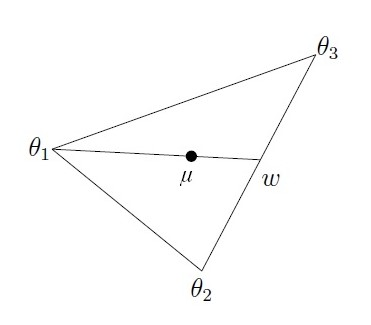
\includegraphics[scale=0.7]{triangle}
\caption{Ilustracija postopka določanja izotropnega vektorja za točko v konveksni ogrinjači treh točk iz $W(A)$.}
\label{fig:triangle}
\end{figure}
Naj bo $\varepsilon >0$ toleranca (npr. $\varepsilon=10^{-16}\norm{A}$ za dvojno natančnost). 
\paragraph{Algoritem:}
\begin{enumerate}[1.]
\item Poiščemo zunanjo aproksimacijo $W(A)$, tako da zračunamo najbolj levo in najbolj desno lastno vrednost $H_\theta =(e^{i\theta}A+e^{-i\theta}A^\ast)/2$ za $\theta =0, \pi/2$. %S tem dobimo zunanjo aproksimacijo zaloge vrednosti, ki seka $\partial W(A)$ v robnih točkah. %RAZLAGA Zunanja aproksimacija bo pravokotnik, katerega stranice so vzporedne z realno in imaginarno osjo. 
Če $\mu$ ni v zunanji aproksimaciji, potem $\mu \not \in W(A)$ in ustavimo algoritem, drugače nadaljujemo.
\item Če je višina ali širina zunanje aproksimacije manj kot $\varepsilon$, potem je $W(A)$ približno hermitska ali poševno-hermitska (ali kompleksen premik katere od teh) in je zaloga vrednosti približno točka. V obeh primerih ugotovimo ali je $\mu \in W(A)$. Če je, poiščemo pripadajoč izotropni vektor. 
\item Če $\mu \not \in W(A)$, nadaljujemo s konstrukcijo notranje aproksimacije $W(A)$ z uporabo lastnih vektorjev najbolj leve in desne lastne vrednosti $H_{\theta}$.% RAZLAGA Notranja aproksimacija bo štirikotnik z oglišči v robnih točkah $\partial W(A)$.
\item  Če $\mu$ leži v notranji aproksimaciji, lahko poiščemo izotropni vektor, ki generira $\mu$. Uporabimo postopek, ki je bil opisan v začetku tega razdelka. %OPISS
Če $\mu$ ne leži v notranji aproksimaciji, določimo katera stranica notranje aproksimacije mu leži najbližje.
\item  Izračunamo $\hat{\mu}$, ki je najbližja točka do $\mu$, ki leži na notranji aproksimaciji. Če je $\abs{\hat{\mu}-\mu}<\varepsilon$, izračunamo izotropni vektor za $\hat{\mu}$ in ga sprejmemo kot izotropni vektor za $\mu$ ter ustavimo algoritem.
\item Posodobimo notranjo in zunanjo aproksimacijo z izračunom največje lastne vrednosti in pripadajočega lastnega vektorja $H_{\theta}$, kjer je smer $\theta$ pravokotna na stranico notranje aproksimacije, ki je najbližja $\mu$. Če ne dobimo nove robne točke, ki se ni dotikala notranje aproksimacije, potem $\mu \not \in W(A)$. 
\item Ponovno preverimo, če je $\mu$  v novi zunanji aproksimaciji. Če je, se vrnemo na 4. korak, drugače $\mu \not \in W(A)$. 
\end{enumerate}
Opomba: Korake 4.-7. ponavljamo, dokler ni notranja aproksimacija $\varepsilon$ blizu $\mu$ ali dokler zunanja aproksimacija ne vsebuje $\mu$. Carden trdi, da se v večini primerov postopek konča v koraku 4. po le nekaj ponavljanjih.\\
Zunanja aproksimacija zaloge vrednosti, ki seka $\partial W(A)$ v robnih točkah, bo pravokotnik, katerega stranice so vzporedne z realno in imaginarno osjo,  notranja aproksimacija pa štirikotnik z oglišči v robnih točkah $\partial W(A)$.
%VKLJUČIM POPRAVEK?
%Ta algoritem ne izkoristi dejstva, da je zaloga vrednosti $2\times2$ matrike elipsa. Ta lastnost nakazuje, da z točkami in pripadajočimi izotropnimi vektorji za notranjo aproksimacijo, lahko natančno določimo izotropne vektorje za točke zunaj notranje aproksimacije. Tako lahko korak 5. popravimo:
%\begin{enumerate}[5.]
%\item Preverimo, če $\mu$ leži na elipsi
%\end{enumerate}
 %Definiraj genarirajoč vektor in ritzove vrednosti
\subsubsection{Chorianopoulos, Psarrakos in Uhlig.}
V tem razdelku opišemo algoritem Chorianopoulosa, Psarrakosa in Uhliga (označimo s CPU) za inverzen problem zaloge vrednosti.
Algoritem je hitrejši in daje natančne numerične rezultate tam, kjer se zgornja algoritma mnogokrat ustavita. Tak primer je ko $\mu$, $\mu \in W(A)$ ali $\mu \not\in W(A)$, leži zelo blizu roba zaloge vrednosti $\partial W(A)$. Ta algoritem uporabi za iskanje izotropnih vektorjev le nekaj najbolj osnovnih lastnosti zaloge vrednosti poleg konveksnosti, kot je $W(\alpha A +\beta I)=\alpha W(A) +\beta$.\\
\paragraph{Algoritem:}
\begin{enumerate}[1.]
\item Izračunamo do 4 robne točke zaloge vrednosti $p_i$ in njihove izotropne vektorje $b_i$, za $i=1,2,3,4$, tako da izračunamo ekstremne lastne vrednosti, ki pripadajo enotskim lastnim vektorjem $x_i$ %a je to isti x oz. b?
matrike $H$ in $K$.
\item Nastavimo $p_i =b^\ast _i Ab_i$. Dobimo 4 točke $p_i$, ki označujejo ekstremne vrednosti $W(A)$, tj. najmanjši in največji horizontalni in vetikalni razteg. Označimo jih z $rM$ in $rm$ za maksimalen in minimalen horizontalni razteg $W(A)$ in z $iM$ in $im$ za maksimalen in minimalen vertikalen razteg $W(A)$.  Če je $|p_i|<10^{-13}$,  za $i=1,2,3,4$, potem je naš izotropni vektor kar pripadajoč enotski vektor.
\item Če med računanjem lastnih vektorjev in lastnih vrednosti ugotovimo, da je ena od matrik $H$ in $iK$ definitna, tj. da imajo njene lastne vrednosti vse enak predznak, potem vemo da $\mu \not\in W(A)$ in algoritem ustavimo.
\item Narišemo elipse, ki so preslikave velikega kroga kompleksne sfere $\C^n$, ki gredo skozi vse možne pare točk $rm, rM, im$ in $iM$, ki imajo nasprotno predznačene imaginarne dele. Nato izračunamo presečišča vsake dobljene elipse z realno osjo.%Poiščemo presečišča realne osi z elipsami, ki so preslikave velikega kroga kompleksne sfere $\C^n$, %ko $x\mapsto x^\ast Ax$, ki grejo skozi vse možne pare izračunanih točk $p_i=x^\ast Ax$, $p_j=y^\ast  Ay$, tj. pari, ki imajo nasprotno predznačene imaginarne dele.
\item Če so izračunana presečišča na obeh straneh 0, potem izračunamo izotropni vektor z lemo \ref{komp}.
\item Če presečišča niso na obeh straneh 0, potem moramo rešiti kvadratno enačbo 
\begin{align}\label{eq:en3}
(tx +(1-t)y)^\ast A(tx+(1-t)y) & =(x^\ast Ax+y^\ast Ay -(x^\ast Ay +y^\ast Ax))t^2 \\
&+(-2y^\ast Ay +(x^\ast Ay+y^\ast Ax))t +y^\ast Ay.\nonumber
\end{align}
Njene ničle določijo koordinatne osi $W(A)$ točk na elipsah skozi točke $x^\ast Ax$, $y^\ast Ay\in \partial W(A)$ %?????
in so generirane s točkami v $\C^n$ na velikem krogu skozi $x$ in $y$. 
\item To je kvadratna enačba s kompleksnimi števili. Nas zanimajo samo rešitve, ki imajo imaginaren del enak 0, saj želimo uporabiti lemo \ref{komp}.
Če imaginarni del enačbe \eqref{eq:en3} enačimo z 0, dobimo naslednjo polinomsko enačbo z realnimi koeficienti:
\begin{equation}
t^2+gt+\frac{p}{f}=0 \label{eq:en4}
\end{equation}
za $q=\Im(x^\ast Ax)$, $p=\Im(y^\ast Ay)$ in $r=\Im(x^\ast  Ay + y^\ast Ax)$. Označimo $f=p+q-r$ in $g=(r-2p)/f$.
\item  Enačba \eqref{eq:en4} ima realni rešitvi $t_i$, $i=1,2$, ki vrneta generirajoča vektorja $b_i=t_ix+(1-t_i)y$ ($i=1,2$) za realni točki. Z normalizacijo dobimo izotropne vektorje. %SLIKA
\item Če nobena od možnih elips ne seka realno os na vsaki strani 0, potem preverimo, če to stori njihova skupna množica in ponovimo isti postopek.
\item Če niti skupna množica ne gre, potem izračunamo še več lastnih vrednosti in lastnih vektorjev za $A(\theta)=\cos(\theta)H+\sin(\theta)iK$ za kote $\theta \not =0,\pi/2$ in delamo bisekcijo med točkami $rm$, $rM$, $im$, $iM$.
\item Končamo, ko najdemo definitno matriko $A(\theta)$ ali elipso, ki seka realno os na obeh straneh 0, nakar lahko uporabimo lemo \ref{komp}.
\end{enumerate}
\section{Numerična analiza}
V tem poglavju bomo primerjali hitrosti algortimov Meuranta (drug algoritem), Cardna in CPU na različnih primerih problema iskanja izotropnih vektorjev. O\-zna\-či\-mo jih z \verb+AlgM+, \verb+AlgC+ in \verb+AlgCPU+. 
%\subsection{Pričakovanjana}
%Za \verb+AlgM+ vemo, da če algoritem potrebuje le 1. korak, deluje hitrejše od ostalih dve algoritmov, saj porabi le eno računanje lastnih vektorjev in vrednosti. Če pa 1. korak ali 2. korak ne delujeta, je to potrata časa in druga dva algoritma delujeta hitreje.
\section{Zaključek}



\vfill

% seznam uporabljene literature
% \cite{meurant} za referenco
\begin{thebibliography}{99}

\bibitem{meurant}
G. Meurant, \emph{The computation of isotropic vectors}, Numer. Alg. {\bf 60} (2012) 193--204.

\bibitem{carden}
R. Carden, \emph{A simple algorithm for the inverse field of values problem}, Inverse Probl. {\bf 25} (2009) 1--9

\bibitem{trije}
C. Chorianopoulos, P. Psarrakos in F. Uhlig, \emph{A method for the inverse numerical range problem}, Electron. J. Linear Algebra {\bf 20} (2010) 198--206

\bibitem{lipkin}
N. Ciblak, H. Lipkin, \emph{Orthonormal isotropic vector bases}, In: Proceedings of DETC'98, 1998 ASME Design Engineering Technical Conferences (1998).

\bibitem{num}
Johnson, C. R., \emph{Numerical determination of the field of values of a general complex matrix}, SIAM J. Numer. Anal. {\bf15} (1978) 595--602.


\end{thebibliography}

\end{document}

